



%%%%%%%%%%%%%%%%%%%%%%%%%%%%%%%%%%%%%%%%%
% Beamer Presentation
% LaTeX Template
% Version 1.0 (10/11/12)
%
% This template has been downloaded from:
% http://www.LaTeXTemplates.com
%
% License:
% CC BY-NC-SA 3.0 (http://creativecommons.org/licenses/by-nc-sa/3.0/)
%
%%%%%%%%%%%%%%%%%%%%%%%%%%%%%%%%%%%%%%%%%

%----------------------------------------------------------------------------------------
%	PACKAGES AND THEMES
%----------------------------------------------------------------------------------------

\documentclass[aspectratio=169]{beamer}

\mode<presentation> {


% The Beamer class comes with a number of default slide themes
% which change the colors and layouts of slides. Below this is a list
% of all the themes, uncomment each in turn to see what they look like.

%\usetheme{default}
%\usetheme{AnnArbor}
%\usetheme{Antibes}
%\usetheme{Bergen}
%\usetheme{Berkeley}
%\usetheme{Berlin}
%\usetheme{Boadilla}
%\usetheme{CambridgeUS}
%\usetheme{Copenhagen}
%\usetheme{Darmstadt}
%\usetheme{Dresden}
%\usetheme{Frankfurt}
%\usetheme{Goettingen}
%\usetheme{Hannover}
%\usetheme{Ilmenau}
%\usetheme{JuanLesPins}
%\usetheme{Luebeck}
\usetheme{Madrid}
%\usetheme{Malmoe}
%\usetheme{Marburg}
%\usetheme{Montpellier}
%\usetheme{PaloAlto}
%\usetheme{Pittsburgh}
%\usetheme{Rochester}
%\usetheme{Singapore}
%\usetheme{Szeged}
%\usetheme{Warsaw}

% As well as themes, the Beamer class has a number of color themes
% for any slide theme. Uncomment each of these in turn to see how it
% changes the colors of your current slide theme.

%\usecolortheme{albatross}
%\usecolortheme{beaver}
%\usecolortheme{beetle}
%\usecolortheme{crane}
%\usecolortheme{dolphin}
%\usecolortheme{dove}
%\usecolortheme{fly}
%\usecolortheme{lily}
%\usecolortheme{orchid}
%\usecolortheme{rose}
%\usecolortheme{seagull}
%\usecolortheme{seahorse}
%\usecolortheme{whale}
%\usecolortheme{wolverine}

%\setbeamertemplate{footline} % To remove the footer line in all slides uncomment this line
%\setbeamertemplate{footline}[page number] % To replace the footer line in all slides with a simple slide count uncomment this line

\definecolor{UOSred}{rgb}{0.6745098039215686, 0.02352941176470588, 0.2039215686274510} % UBC Blue (primary)
\definecolor{UOSgrey}{rgb}{0.8117647058823529, 0.8117647058823529, 0.8117647058823529} % UBC Grey (secondary)

\setbeamercolor{palette primary}{bg=UOSred,fg=white}
\setbeamercolor{palette secondary}{bg=UOSred,fg=white}
\setbeamercolor{palette tertiary}{bg=UOSred,fg=white}
\setbeamercolor{palette quaternary}{bg=UOSred,fg=white}
\setbeamercolor{structure}{fg=UOSred} % itemize, enumerate, etc
\setbeamercolor{section in toc}{fg=UOSred} % TOC sections

%gets rid of bottom navigation bars
\setbeamertemplate{footline}[frame number]{}

%gets rid of bottom navigation symbols
\setbeamertemplate{navigation symbols}{}


\usepackage{amsmath}
\usepackage{selinput}      % Halbautomatische Auswahl der Eingabecodierung
\SelectInputMappings{      % mit Hilfe ausgewählter Glyphen
  adieresis={ä},	   % siehe: http://partners.adobe.com/public/developer/en/opentype/glyphlist.txt
  germandbls={ß},
  Euro={€}
}

\addtobeamertemplate{footline}{%
  \leavevmode%
  \hbox{%
  \begin{beamercolorbox}[wd=\paperwidth,ht=2.25ex,dp=1ex,center]{author in head/foot}%
     \insertsectionnavigationhorizontal{\paperwidth}{}{}
  \end{beamercolorbox}}%

}

% Override palette coloring with secondary
\setbeamercolor{subsection in head/foot}{bg=UOSgrey,fg=white}

%\setbeamertemplate{navigation symbols}{} % To remove the navigation symbols from the bottom of all slides uncomment this line
}
\usepackage{hyperref}
\usepackage{graphicx} % Allows including images
\usepackage{grffile}
\usepackage{booktabs} % Allows the use of \toprule, \midrule and \bottomrule in tables
\graphicspath{{images/}}
%----------------------------------------------------------------------------------------
%	TITLE PAGE
%----------------------------------------------------------------------------------------

\title[Übungsprojekt Phase 4]{Übungsprojekt Phase 4} % The short title appears at the bottom of every slide, the full title is only on the title page

\author{T. Adam, M. ben Ahmed} % Your name
\institute[UOS] % Your institution as it will appear on the bottom of every slide, may be shorthand to save space
{

Universität Osnabrück \\ % Your institution for the title page

\medskip
\textit{Æ} % Your email address


}
\date{\today} % Date, can be changed to a custom date

\begin{document}

\begin{frame}
\titlepage % Print the title page as the first slide
\end{frame}


%----------------------------------------------------------------------------------------
%	PRESENTATION SLIDES
%----------------------------------------------------------------------------------------


%------------------------------------------------
\begin{frame}
\frametitle{Phase 4 - Simulated Annealing}
\begin{columns}[c] % The "c" option specifies centered vertical alignment while the "t" option is used for top vertical alignment
	
	\column{.6\textwidth} % Left column and width
	\textbf{Verbesserung von Simulated Annealing}
	\begin{itemize}
		\item Simulated Annealing hat unter den Heuristiken die besten Lösungen geliefert
		\item Bietet viel Raum für Verbesserungen an
		\item Nähert die optimale Lösung beliebig nahe an
	\end{itemize}
	\column{.3\textwidth} % Right column and width
\end{columns}
\end{frame}
%------------------------------------------------

\begin{frame}
\frametitle{Phase 4 - Simulated Annealing}
\begin{columns}[c] % The "c" option specifies centered vertical alignment while the "t" option is used for top vertical alignment
	\column{.55\textwidth} % Left column and width
	\textbf{Simulated Annealing:}
	\begin{itemize}
		\item Es werden Nachbarschaften von Lösungen  betrachtet
		\item Bessere und gleiche Lösungen werden immer akzeptiert
		\item Verschlechterungen werden mit bestimmter Wahrscheinlichkeit akzeptiert
	\end{itemize}
	\column{.45\textwidth} % Right column and width
	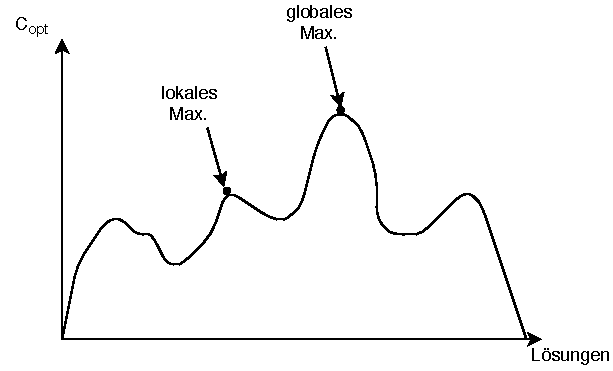
\includegraphics[scale=.6]{sa_maximum.pdf}	
\end{columns}
\end{frame}

%------------------------------------------------

\begin{frame}
\frametitle{Phase 4 - Verbesserungen}
\textbf{Änderungen zu Phase 2}\\
\begin{itemize}
	\item Effiziente Datenstruktur für Konflikterkennung
	\begin{itemize}
		\item[$\rightarrow$] Potenzielle Konflikte für jeden Punkt speichern
	\end{itemize}
	\item Implementation eines Parameter Tuning Tools
	\begin{itemize}
		\item[$\rightarrow$] Parameter mittels Bayesian Optimization finden
	\end{itemize}
	\item Hinzufügen mehrerer neuer Nachbarschaften
\end{itemize}
\end{frame}

%------------------------------------------------

\begin{frame}
\frametitle{Phase 4 - Verbesserungen}
\textbf{Bayesian Optimization}\\
\begin{itemize}
	\item Versucht das maximum einer Funktion zu finden
	\item $\underset{x \in A}{\max} \thinspace f(x)$ mit $x \in \mathbb{R}^d$
	\item Gut geeignet für Funktionen $f$ die viel Zeit zum berechnen brauchen
	\item Ableitungen müssen nicht bekannt sein, $f$ als "Black-Box"
	\item Hier: $f(x) = SimulatedAnnealing(parameter) $
\end{itemize}
\end{frame}

%------------------------------------------------

\begin{frame}
\frametitle{Phase 4 - Verbesserungen}
\begin{columns}[c] % The "c" option specifies centered vertical alignment while the "t" option is used for top vertical alignment
	
	\column{.45\textwidth} % Left column and width
	\textbf{Nachbarschaft 1}
	\begin{itemize}
		\item ein zufälliger Punkt wird gewählt
		\item Label wird hinzugefügt/geändert/gelöscht
		\item[]
		\item[]
		\item[]
	\end{itemize}
	
	\column{.45\textwidth} % Right column and width
	\textbf{Nachbarschaft 2}
	\begin{itemize}
		\item ein zufälliger Punkt wird gewählt
		\item Label wird gelöscht
		\item Label aller potentiellen Konfliktpunkte werden geändert
		\item[]
		\item[]
	\end{itemize}
\end{columns}
\centering
	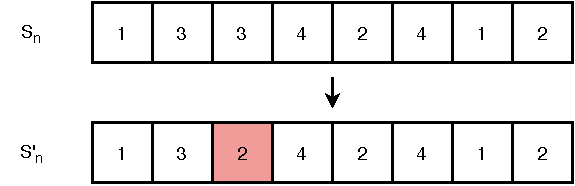
\includegraphics[scale=.6]{sa_representation.pdf}

\end{frame}

%------------------------------------------------
\begin{frame}
\frametitle{Ergebnisse}
\textbf{Parameter Tuning Tool}

\begin{itemize}
	\item Manuell bestimmte Parameter konnten nicht signifikant verbessert werden
	\item Für Nachbarschaft 2 haben einige Parameter wenig Einfluss
	\item[]
	\item Mögliche Ursachen: 
	\begin{itemize}
		\item Zu starke schwankungen durch Zufall
		\item Zu wenige Iterationen des Optimizers
	\end{itemize}
\end{itemize}

\end{frame}
%------------------------------------------------

\begin{frame}
\frametitle{Ergebnisse}
\begin{columns}[c] % The "c" option specifies centered vertical alignment while the "t" option is used for top vertical alignment
	
	\column{.30\textwidth} % Left column and width
	\textbf{Intel Core i5-3570K}
	\begin{itemize}
		\item 4c/4t
		\item 3,4 - 3,8 GHz
		\item 6 MB L3
		\item 16 GB (1600 MHz)
		\item Linux (Kubuntu 18.04)
	\end{itemize}
	
	\column{.30\textwidth} % Right column and width
	\textbf{Intel Core i7-3770K}
	\begin{itemize}
		\item 4c/8t
		\item 3,5 - 3,9 GHz
		\item 8 MB L3
		\item 16 GB (1600 MHz)
		\item Linux (Kubuntu 18.04)
		
	\end{itemize}
\end{columns}
\end{frame}

%------------------------------------------------


\begin{frame}
\frametitle{Phase 4 - Ergebnisse}
\begin{columns}[c] % The "c" option specifies centered vertical alignment while the "t" option is used for top vertical alignment
	
	\column{.45\textwidth} % Left column and width
	\textbf{Ergebnisse}
	\begin{itemize}
		\item Deutliche Verbesserung der Laufzeit
	\end{itemize}
	\column{.45\textwidth} % Right column and width
	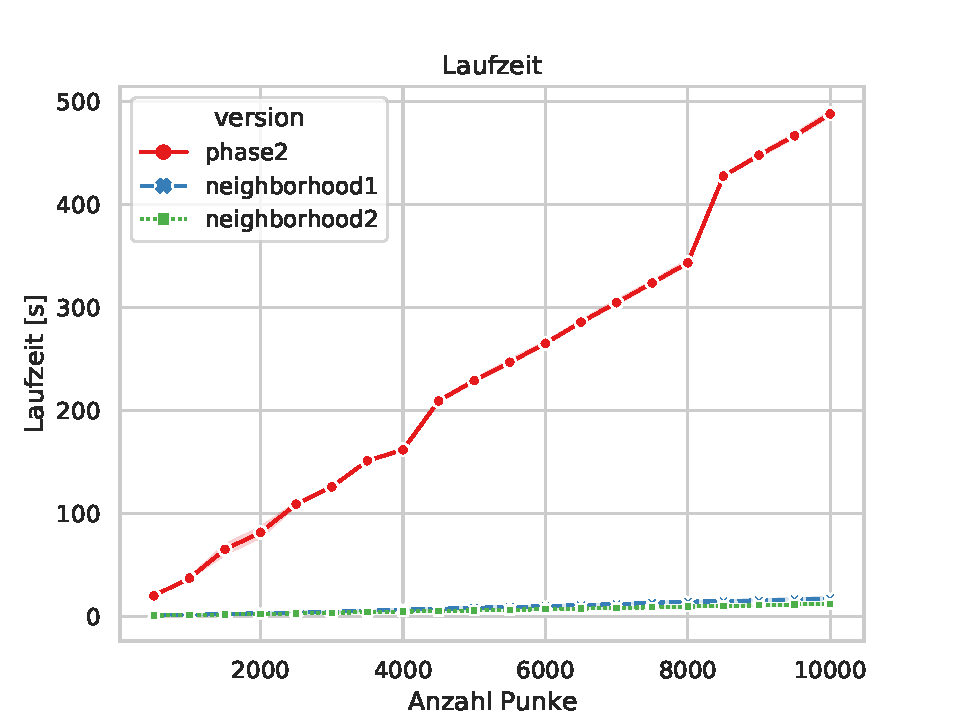
\includegraphics[scale=.45]{runtime_overview.pdf}	
\end{columns}
\end{frame}

%------------------------------------------------

\begin{frame}
\frametitle{Phase 4 - Ergebnisse}
\begin{columns}[c] % The "c" option specifies centered vertical alignment while the "t" option is used for top vertical alignment
	
	\column{.45\textwidth} % Left column and width
	\textbf{Ergebnisse}
	\begin{itemize}
		\item Nachbarschaft 2 lässt sich schneller Berechnen als Nachbarschaft 1
	\end{itemize}
	\column{.45\textwidth} % Right column and width
	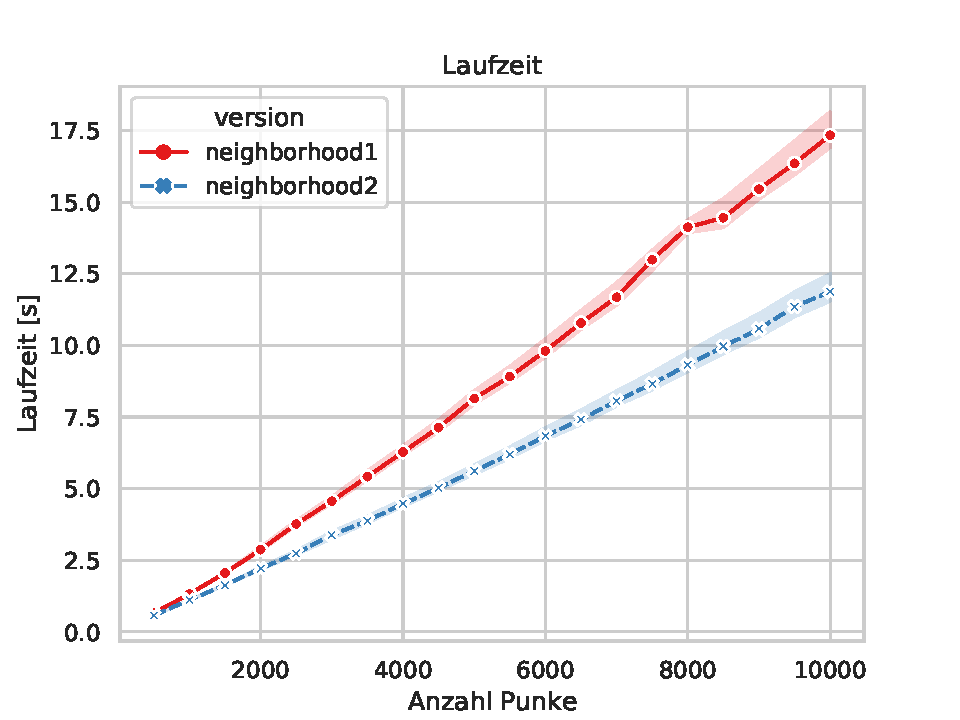
\includegraphics[scale=.45]{runtime_neighborhood.pdf}	
\end{columns}
\end{frame}

%------------------------------------------------

\begin{frame}
\frametitle{Phase 4 - Ergebnisse}
\begin{columns}[c] % The "c" option specifies centered vertical alignment while the "t" option is used for top vertical alignment
	
	\column{.45\textwidth} % Left column and width
	\textbf{Ergebnisse}
	\begin{itemize}
		\item Nachbarschaft 2 liefert bei größeren Instanzen bessere Ergebnisse
		\item bei kleinen Instanzen ist Nachbarschaft 1 leicht besser
		\item Ziefunktionswert aus Phase 2 fast identisch zu Nachbarschaft 1
	\end{itemize}
	\column{.45\textwidth} % Right column and width
	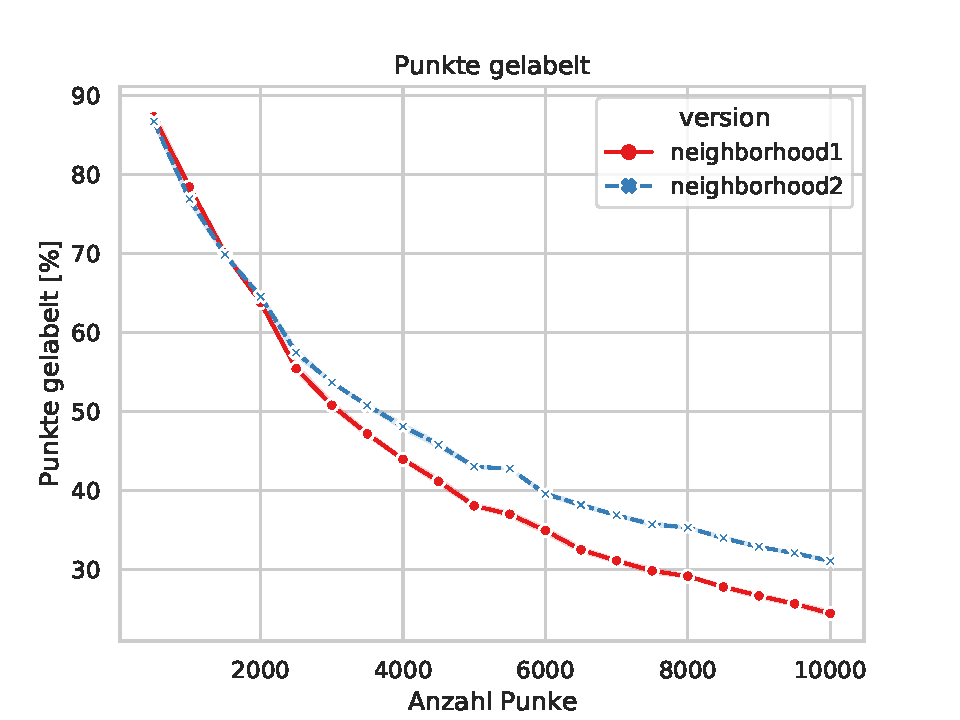
\includegraphics[scale=.45]{sol_neighborhood.pdf}	
\end{columns}
\end{frame}

%------------------------------------------------

\begin{frame}
\frametitle{Ergebnisse}
\textbf{Zusammenfassung}

\begin{itemize}
	\item Parameter Tuning Tool konnte nicht sinnvoll eingesetzt werden
	\item Laufzeit konnte um vielfaches reduziert werden
	\item Erreichte Zielfunktionswerte um mehrere Prozent gesteigert
	\item[]
	\item Parameter zeigen viel Potential für weitere Verbesserungen
	\item Gute Parameter schwierig zu finden
\end{itemize}

\end{frame}


\end{document} 